\chapter{T-05: Cortes por plataforma y contexto}

\section{Objetivo}

Consolidar métricas oficiales por cortes demográficos y contextuales a partir de las predicciones T-04, con normalización \texttt{SI/SÍ/NO} y advertencias de baja potencia en slices pequeños.

\section{Cortes generales}

\begin{table}[H]
  \centering
  \caption{F1-macro por corte contextual}
  \label{tab:slices}
  \begin{tabular}{lllrrccc}
\toprule
Modelo & Corte & Definición & n & Clases & F1-macro & IC / nota & Accuracy \\
\midrule
mBERT & con\_jerga & n\_jerga > 0 & 278 & 29/117/72/60 & 0.7632 & [0.7028, 0.8171] & 0.7950 \\
mBERT & contexto\_politico\_no & Contexto\_Politico in \{NO/FALSE/0/N\} & 368 & 107/97/93/71 & 0.7608 & [0.7201, 0.8036] & 0.7609 \\
mBERT & contexto\_politico\_si & Contexto\_Politico in \{SI/SÍ/YES/TRUE/1\} & 92 & 16/62/2/12 & 0.7875 & baja potencia: clase con n<5 & 0.8696 \\
mBERT & ironia\_no & Presencia\_Ironia in \{NO/FALSE/0/N\} & 401 & 94/136/88/83 & 0.7871 & [0.7469, 0.8258] & 0.7880 \\
mBERT & ironia\_si & Presencia\_Ironia in \{SI/SÍ/YES/TRUE/1\} & 59 & 29/23/7/0 & 0.5247 & baja potencia: faltan clases (n=59) & 0.7458 \\
mBERT & plataforma\_Facebook & Plataforma == 'Facebook' & 232 & 75/88/30/39 & 0.6727 & [0.5978, 0.7370] & 0.7241 \\
mBERT & plataforma\_X & Plataforma == 'X' & 228 & 48/71/65/44 & 0.8386 & [0.7903, 0.8851] & 0.8421 \\
mBERT & sarcasmo\_no & Presencia\_Sarcasmo in \{NO/FALSE/0/N\} & 370 & 91/111/87/81 & 0.7923 & [0.7496, 0.8296] & 0.7919 \\
mBERT & sarcasmo\_si & Presencia\_Sarcasmo in \{SI/SÍ/YES/TRUE/1\} & 90 & 32/48/8/2 & 0.5881 & baja potencia: clase con n<5 & 0.7444 \\
mBERT & sin\_jerga & n\_jerga == 0 & 182 & 94/42/23/23 & 0.6893 & [0.6059, 0.7647] & 0.7637 \\
\bottomrule
\end{tabular}

\end{table}

\begin{figure}[H]
  \centering
  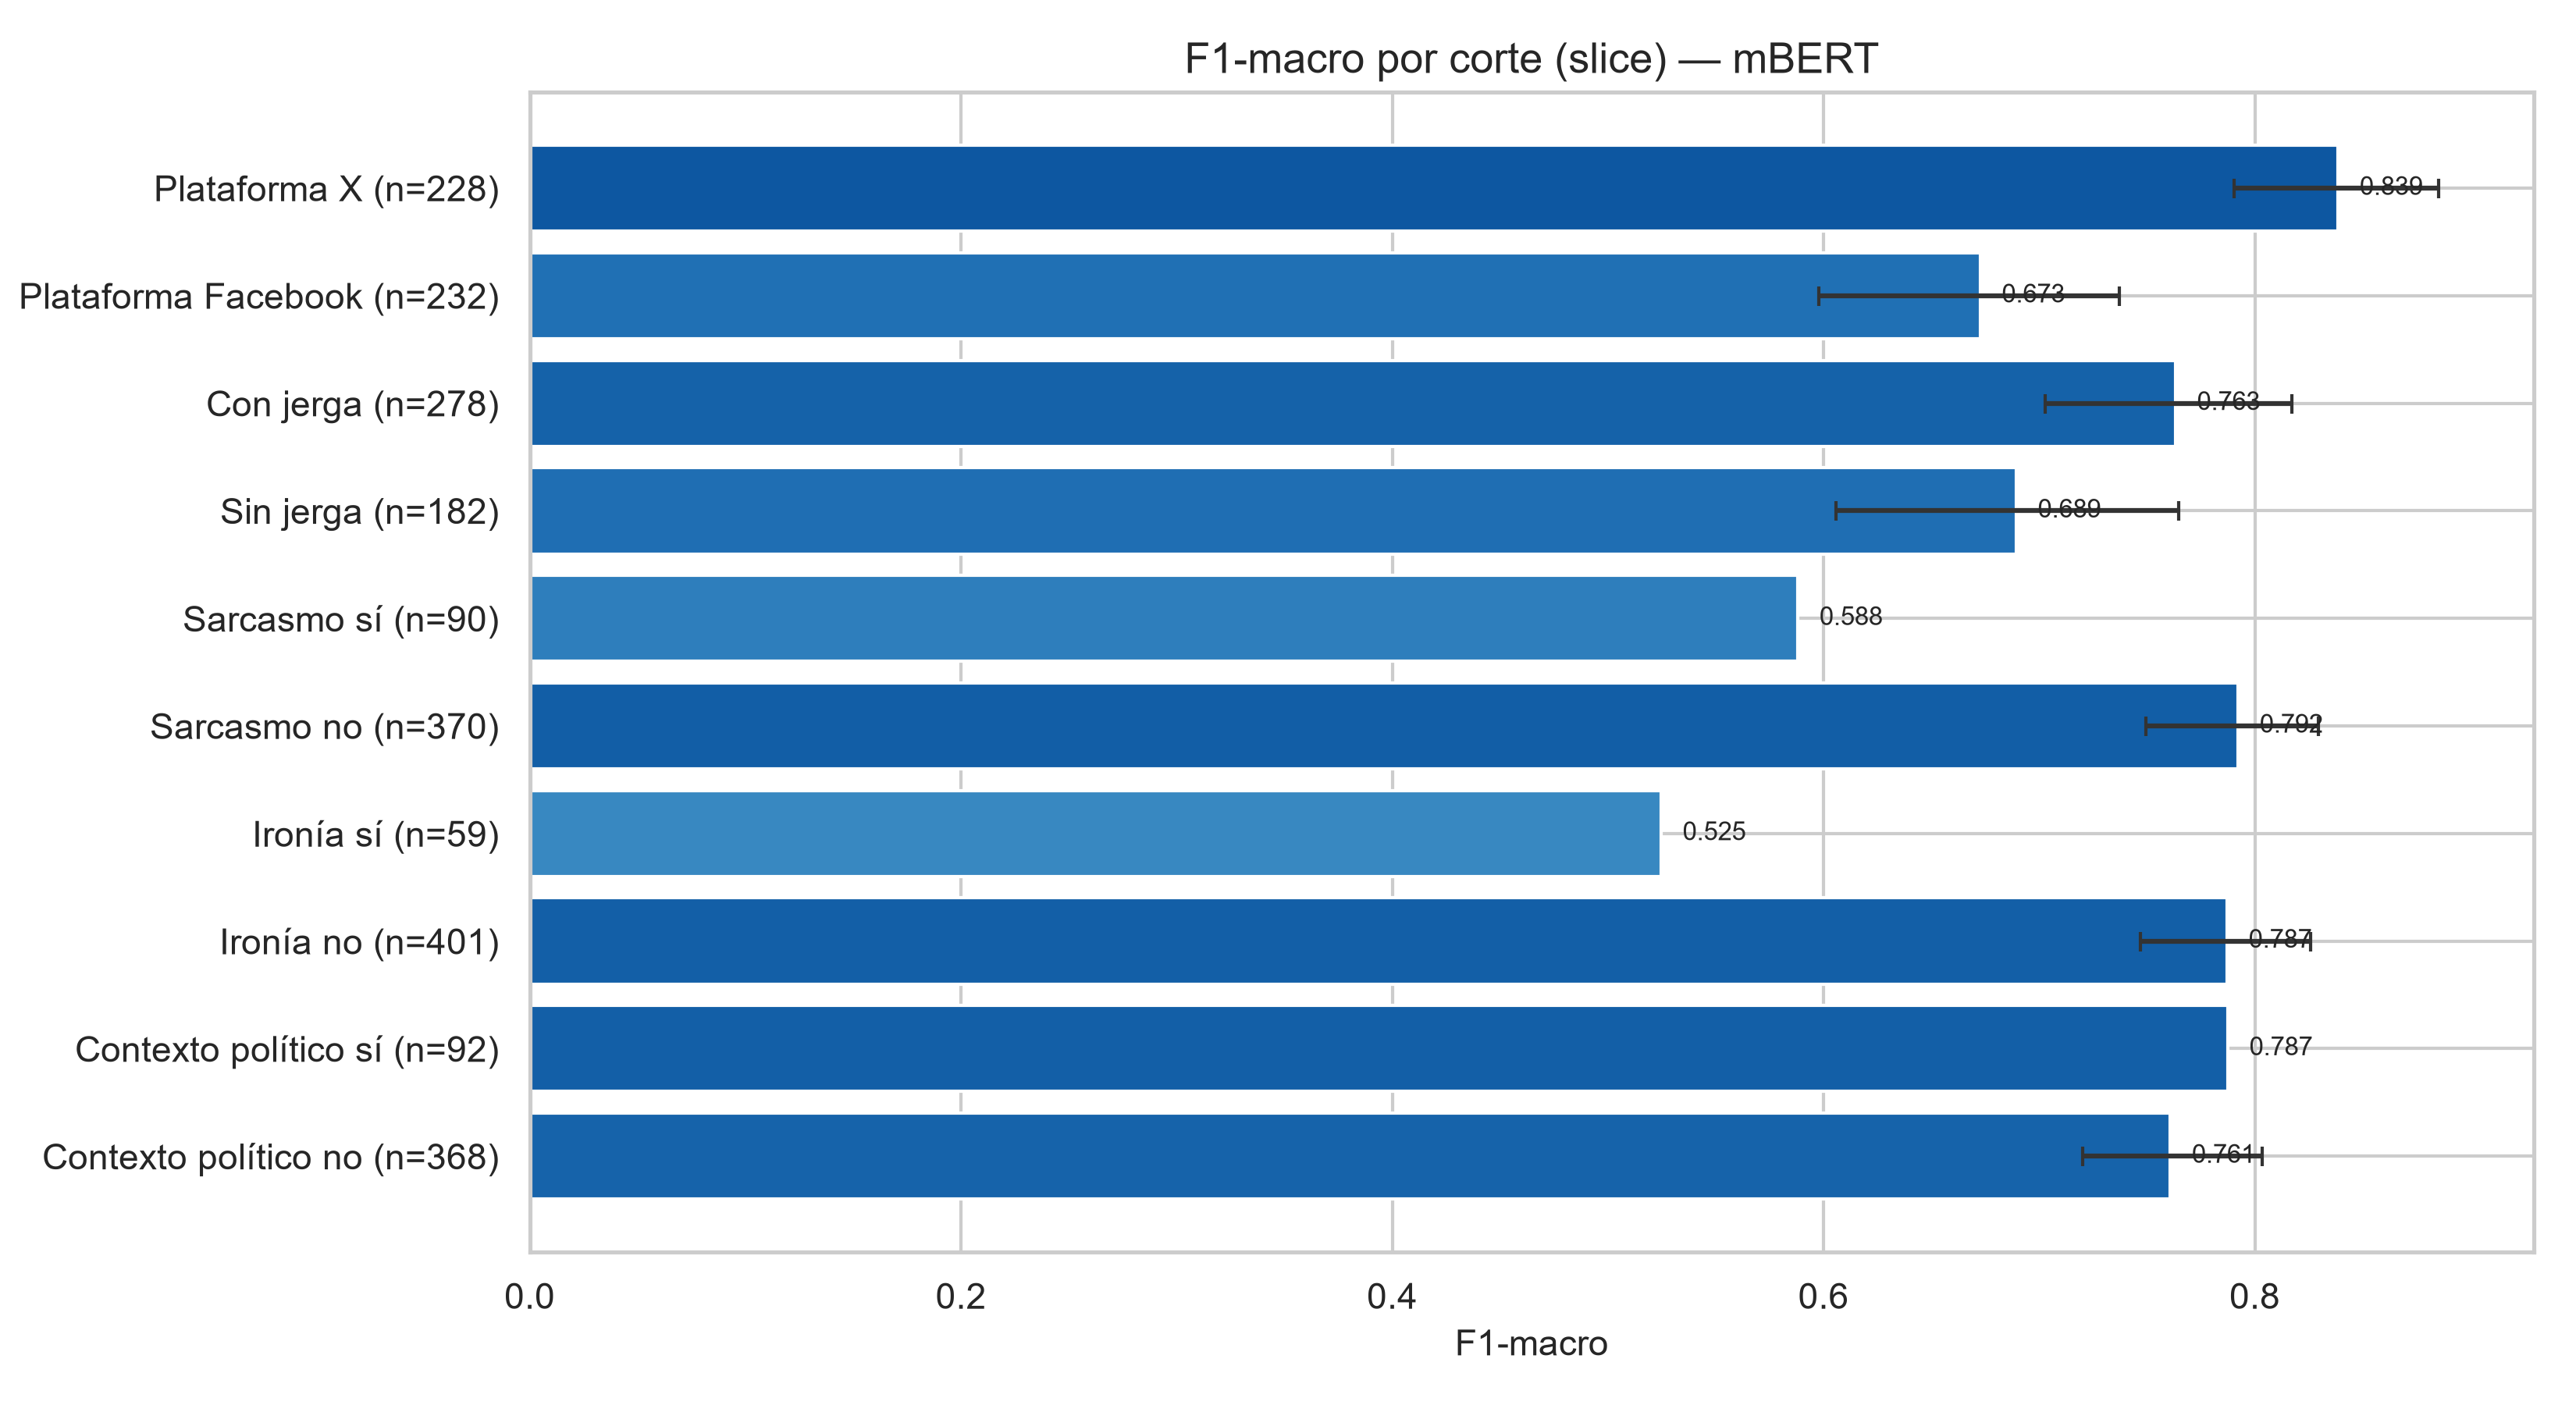
\includegraphics[width=0.85\textwidth]{07_slice_f1_heatmap.png}
  \caption{Mapa de calor F1-macro por corte}
  \label{fig:slices}
\end{figure}

\section{Plataforma}

\begin{table}[H]
  \centering
  \caption{F1-macro por plataforma (mBERT oficial)}
  \label{tab:platform}
  \begin{tabular}{lllrrrrc}
\toprule
Modelo & Plataforma & Checkpoint & n & Clases & F1-macro & Accuracy & IC / nota \\
\midrule
mBERT & Facebook & checkpoint-1072 & 232 & 75/88/30/39 & 0.6727 & 0.7241 & [0.5978, 0.7370] \\
mBERT & X & checkpoint-1072 & 228 & 48/71/65/44 & 0.8386 & 0.8421 & [0.7903, 0.8851] \\
XLM-RoBERTa & Facebook & xlmr\_test\_predictions.csv & 232 & 75/88/30/39 & 0.7154 & 0.7457 & [0.6435, 0.7764] \\
XLM-RoBERTa & X & xlmr\_test\_predictions.csv & 228 & 48/71/65/44 & 0.8673 & 0.8684 & [0.8216, 0.9116] \\
\bottomrule
\end{tabular}

\end{table}

\begin{figure}[H]
  \centering
  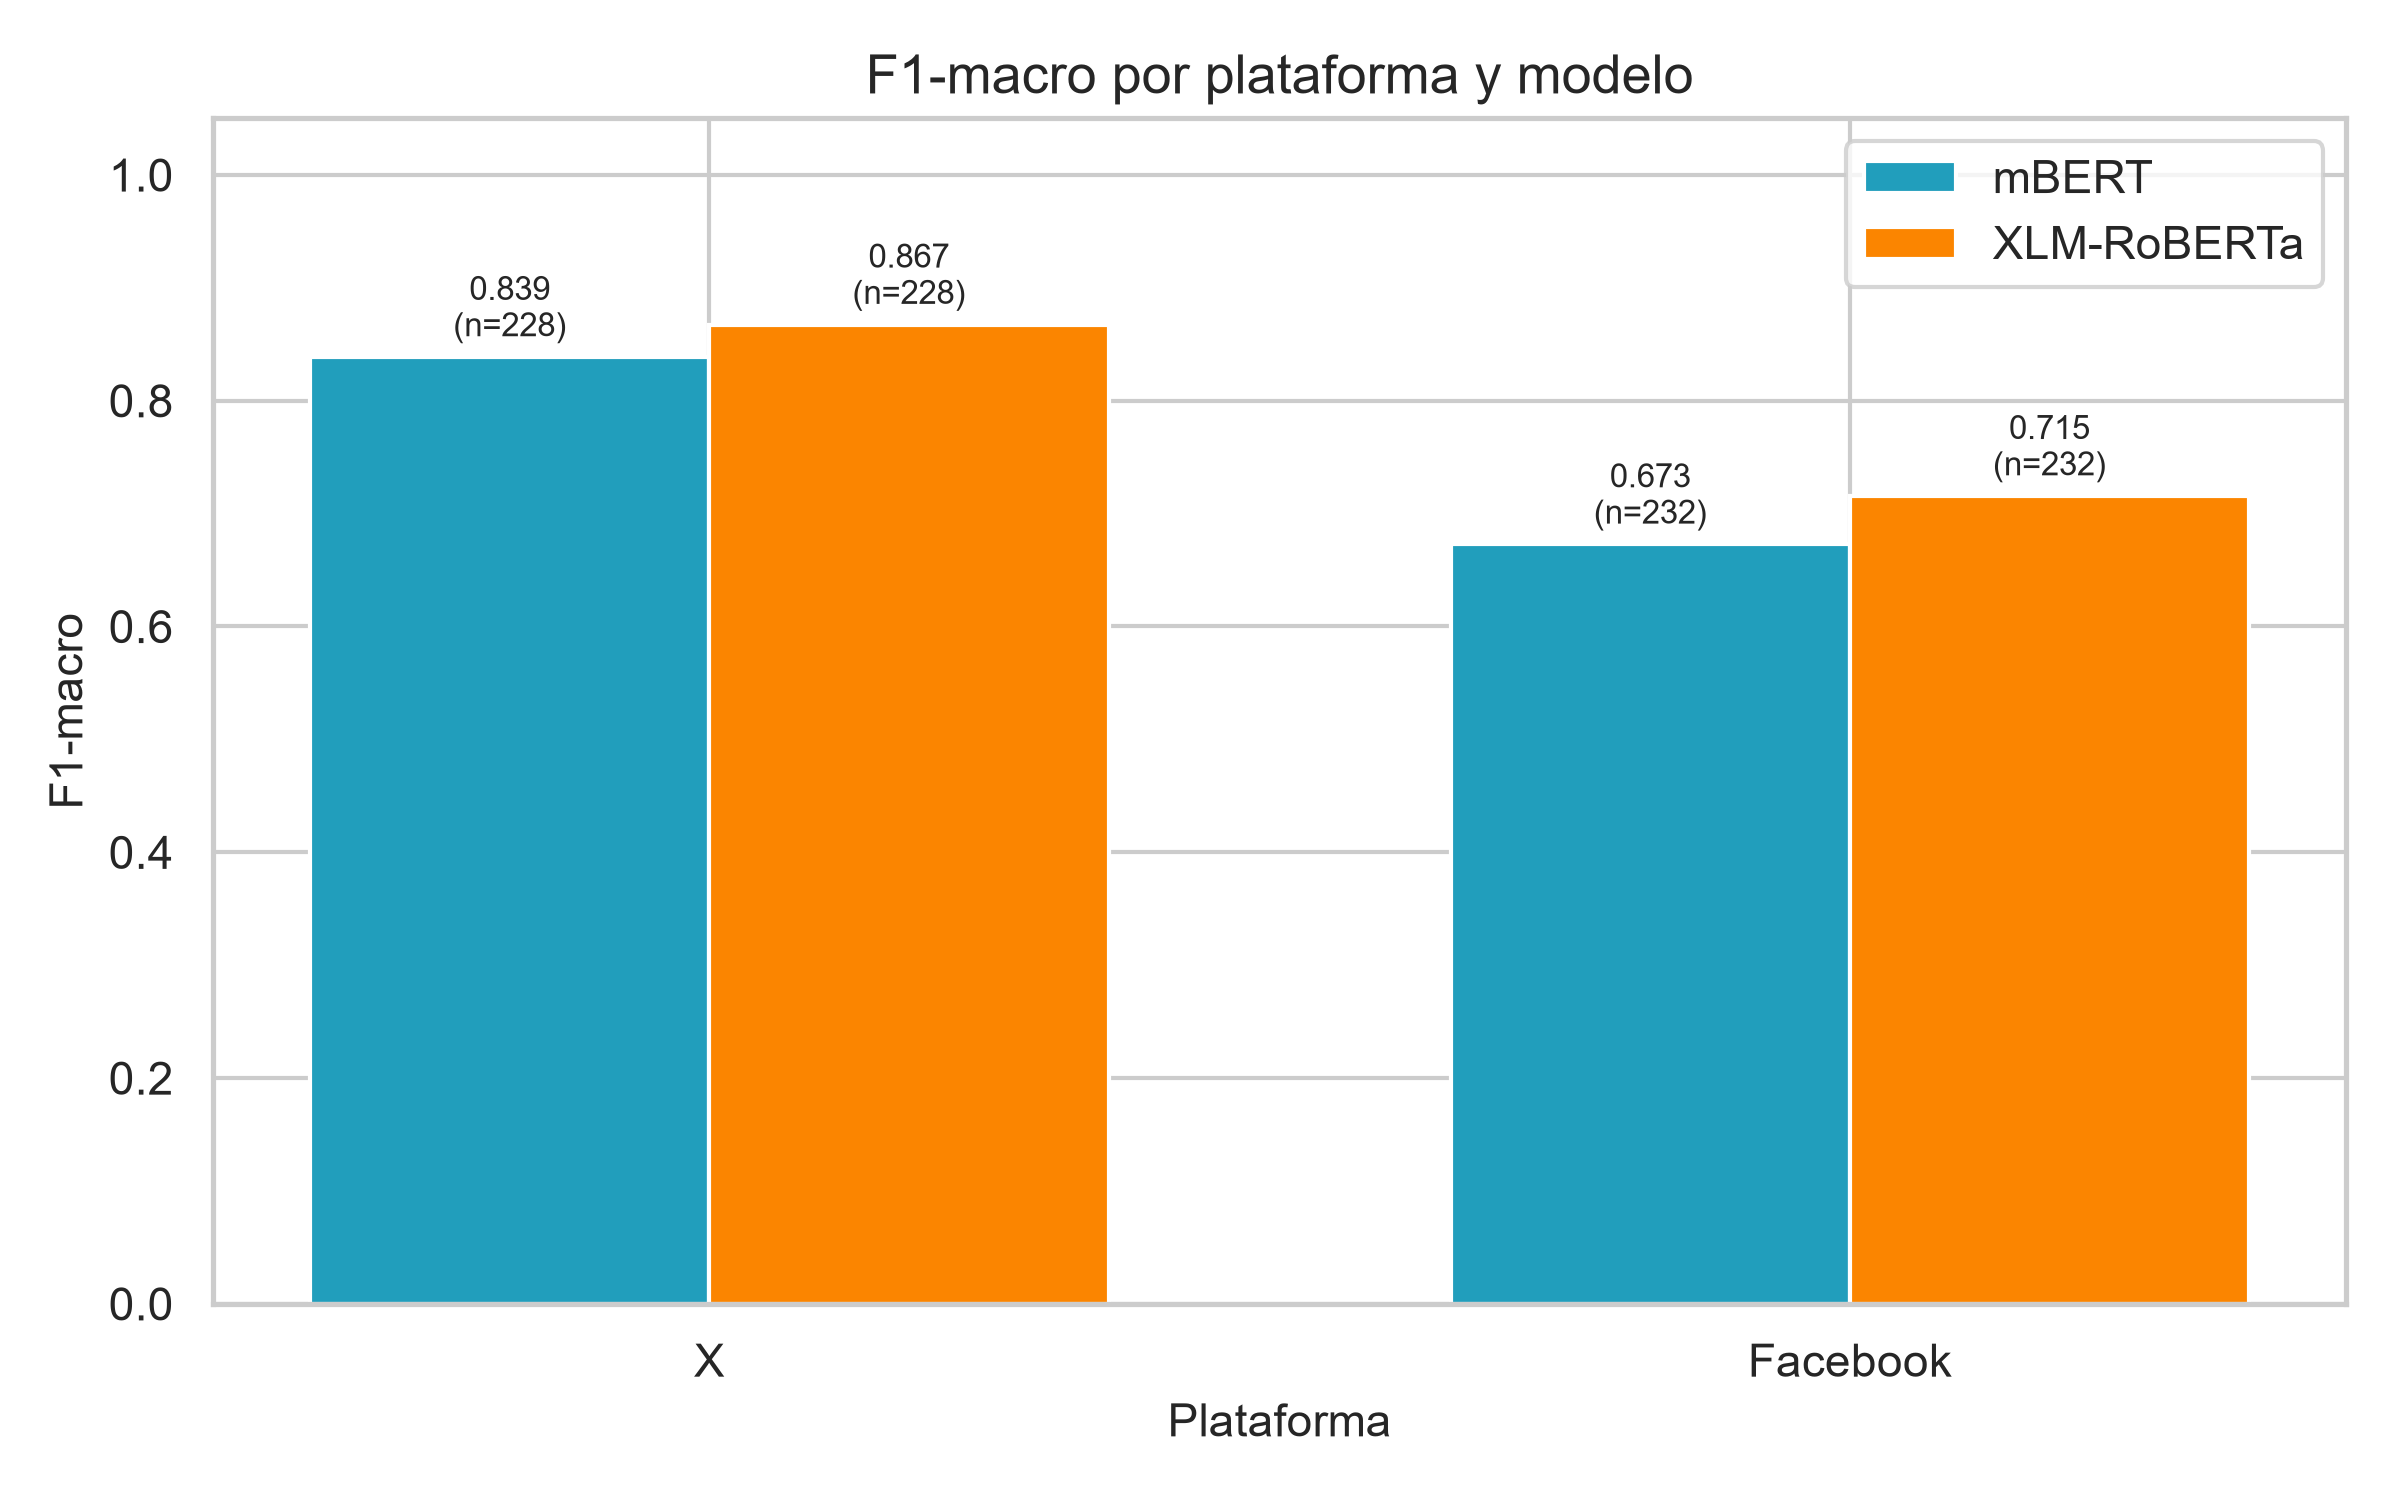
\includegraphics[width=0.75\textwidth]{08_platform_f1_grouped.png}
  \caption{Comparación F1-macro por plataforma}
  \label{fig:platform}
\end{figure}

Destacan brechas entre X (F1 $\approx$ 0.84) y Facebook (F1 $\approx$ 0.67).

\section{Sonda de sesgo dialectal (test principal)}

\begin{table}[H]
  \centering
  \caption{Sonda de sesgo dialectal en test ($n=460$)}
  \label{tab:dialect-bias}
  \begin{tabular}{llccccr}
\toprule
Modelo & Grupo & FP/n & FPR & IC 95\% lo & IC 95\% hi & n \\
\midrule
mbert & Con jerga & 12/29 & 0.4138 & 0.2551 & 0.5926 & 29 \\
mbert & Sin jerga & 15/94 & 0.1596 & 0.0992 & 0.2467 & 94 \\
xlm-roberta & Con jerga & 13/29 & 0.4483 & 0.2841 & 0.6245 & 29 \\
xlm-roberta & Sin jerga & 15/94 & 0.1596 & 0.0992 & 0.2467 & 94 \\
\bottomrule
\end{tabular}

\end{table}

\begin{figure}[H]
  \centering
  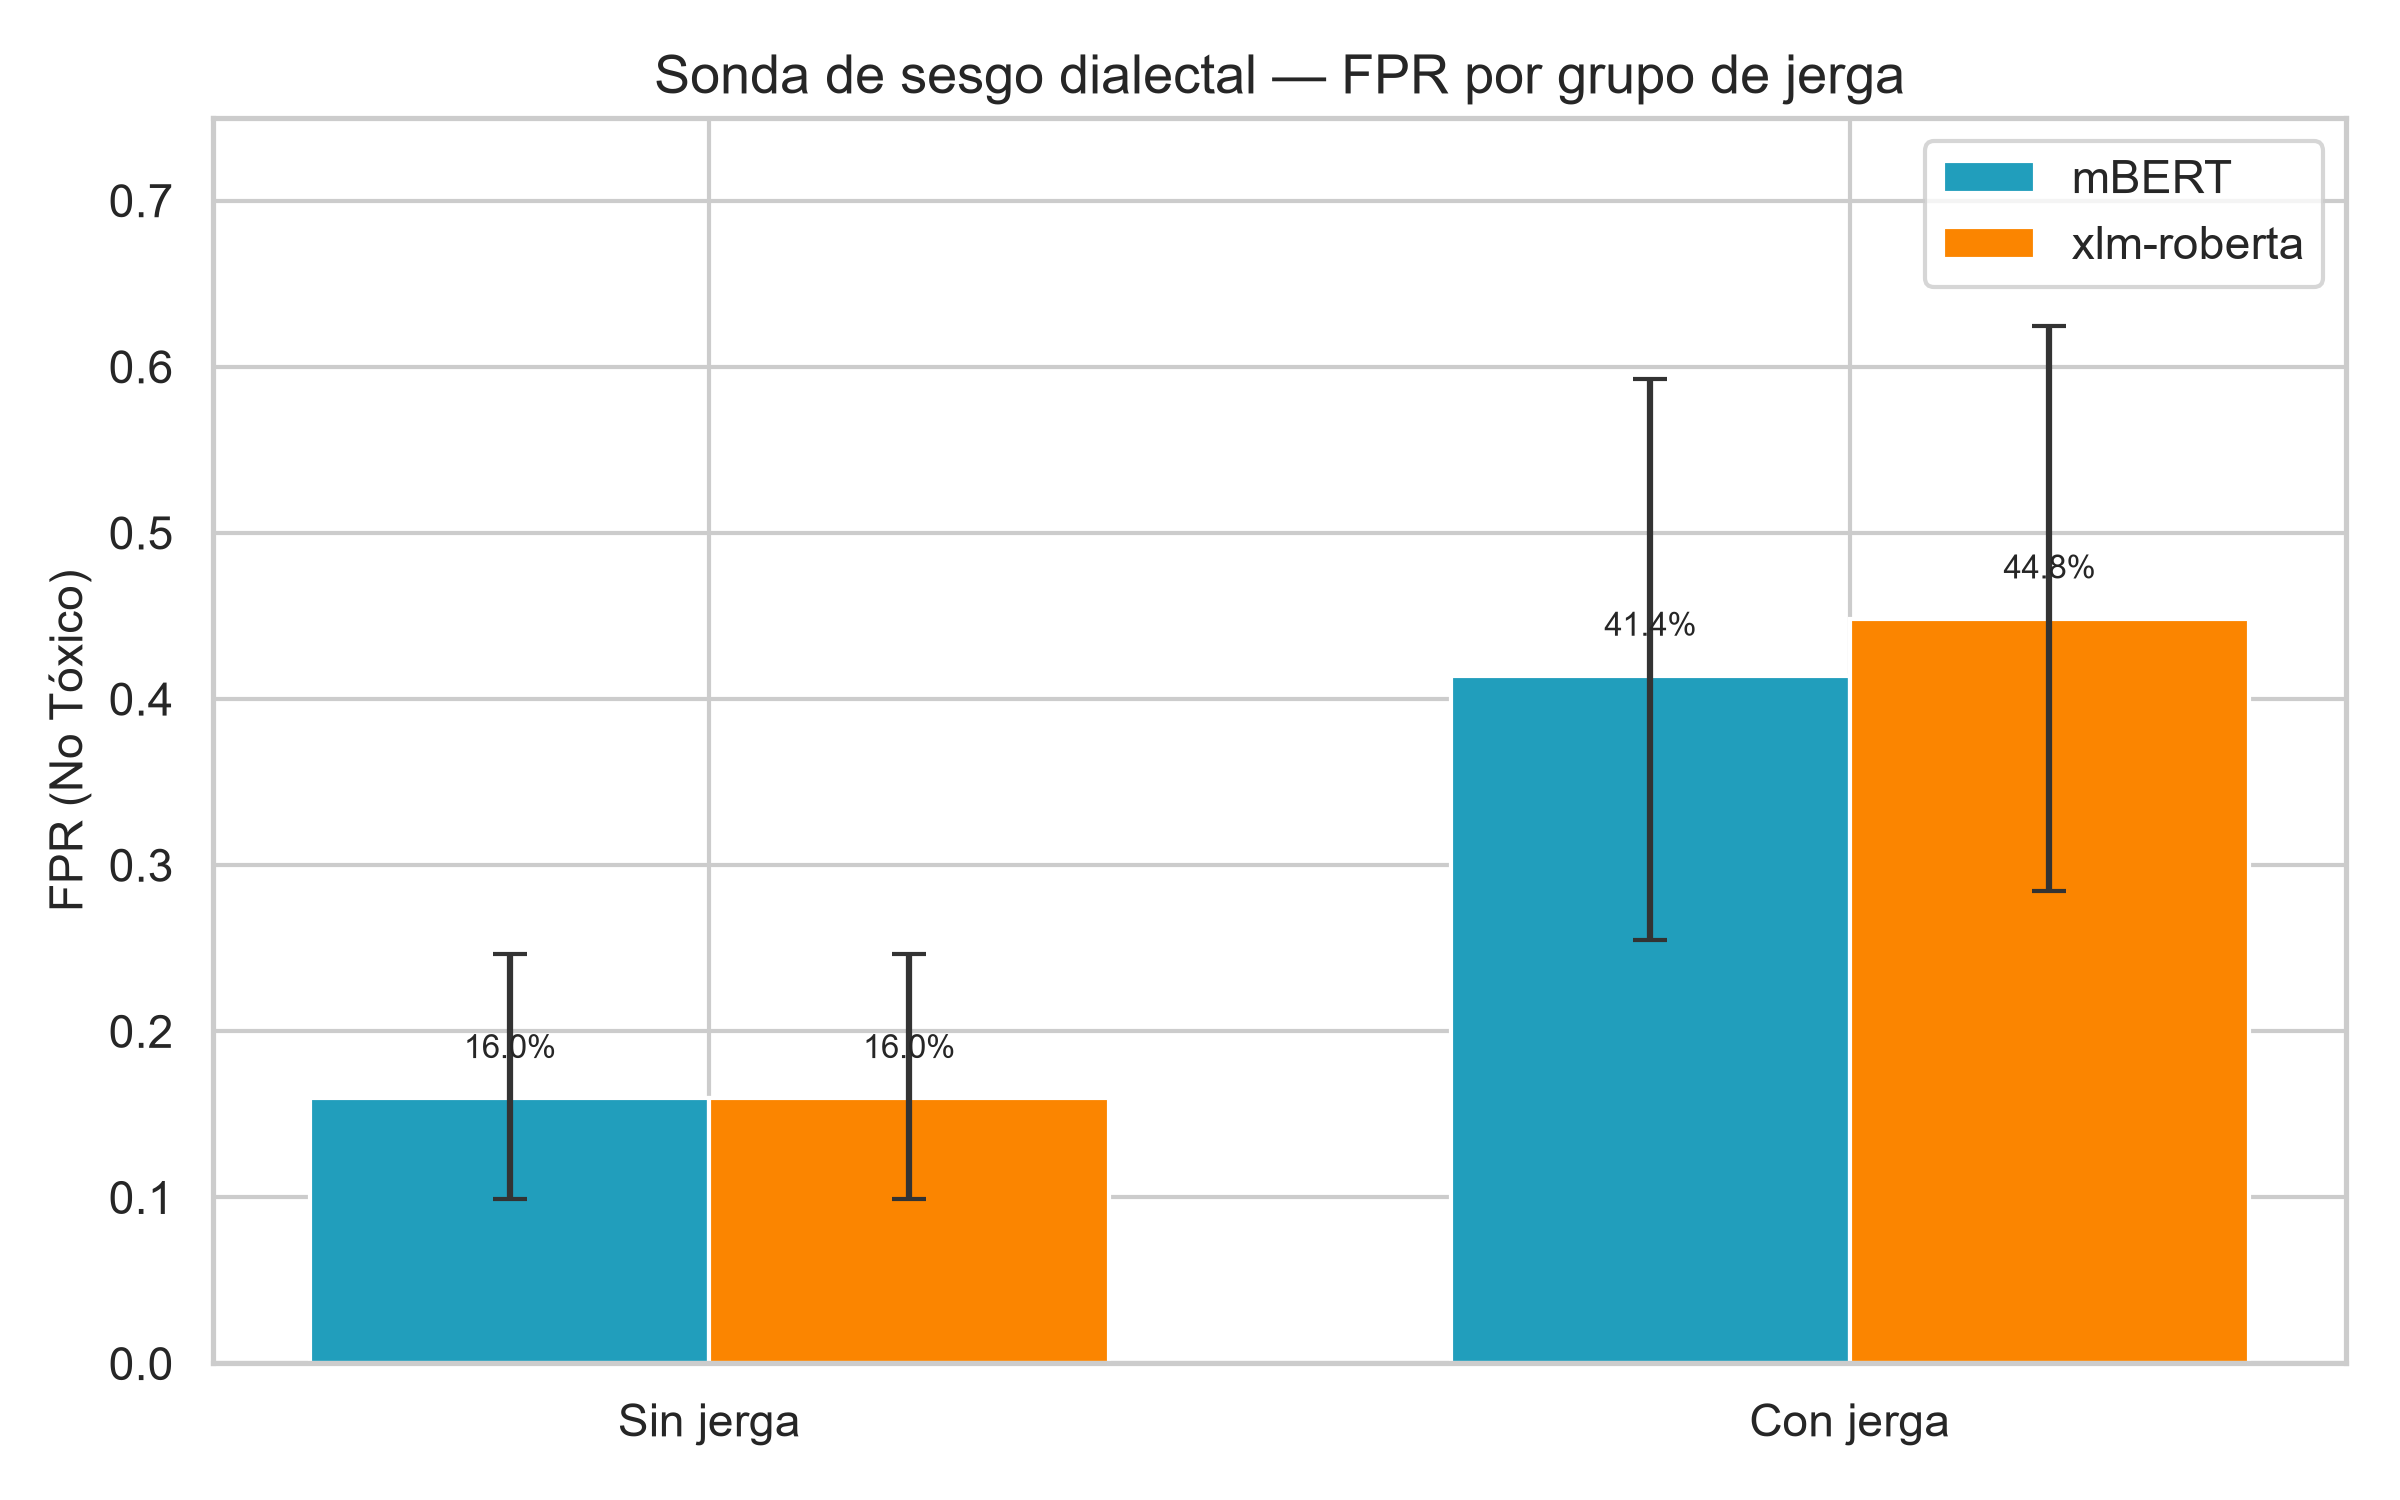
\includegraphics[width=0.7\textwidth]{10_dialect_bias_fpr.png}
  \caption{FPR en No Tóxico: con vs sin jerga salvadoreña}
  \label{fig:dialect-fpr}
\end{figure}

\textbf{Criterio de cierre:} \texttt{slice\_metrics.csv}, \texttt{dialect\_bias\_probe.csv} y tablas LaTeX regeneradas desde CSV; tests en \texttt{test\_mbert\_slices\_official.py}.
